\documentclass[]{article}
\usepackage{lmodern}
\usepackage{amssymb,amsmath}
\usepackage{ifxetex,ifluatex}
\usepackage{fixltx2e} % provides \textsubscript
\ifnum 0\ifxetex 1\fi\ifluatex 1\fi=0 % if pdftex
  \usepackage[T1]{fontenc}
  \usepackage[utf8]{inputenc}
\else % if luatex or xelatex
  \ifxetex
    \usepackage{mathspec}
  \else
    \usepackage{fontspec}
  \fi
  \defaultfontfeatures{Ligatures=TeX,Scale=MatchLowercase}
\fi
% use upquote if available, for straight quotes in verbatim environments
\IfFileExists{upquote.sty}{\usepackage{upquote}}{}
% use microtype if available
\IfFileExists{microtype.sty}{%
\usepackage{microtype}
\UseMicrotypeSet[protrusion]{basicmath} % disable protrusion for tt fonts
}{}
\usepackage[margin=1in]{geometry}
\usepackage{hyperref}
\hypersetup{unicode=true,
            pdftitle={A template for writing a manuscript in Rmarkdown},
            pdfauthor={W. J. Grecian1, I. D. Jonsen2; 1Sea Mammal Research Unit, Scottish Oceans Institute, University of St Andrews, St Andrews, UK; 2Dept. of Biological Sciences, Macquarie University, Sydney, Australia},
            pdfborder={0 0 0},
            breaklinks=true}
\urlstyle{same}  % don't use monospace font for urls
\usepackage{longtable,booktabs}
\usepackage{graphicx,grffile}
\makeatletter
\def\maxwidth{\ifdim\Gin@nat@width>\linewidth\linewidth\else\Gin@nat@width\fi}
\def\maxheight{\ifdim\Gin@nat@height>\textheight\textheight\else\Gin@nat@height\fi}
\makeatother
% Scale images if necessary, so that they will not overflow the page
% margins by default, and it is still possible to overwrite the defaults
% using explicit options in \includegraphics[width, height, ...]{}
\setkeys{Gin}{width=\maxwidth,height=\maxheight,keepaspectratio}
\IfFileExists{parskip.sty}{%
\usepackage{parskip}
}{% else
\setlength{\parindent}{0pt}
\setlength{\parskip}{6pt plus 2pt minus 1pt}
}
\setlength{\emergencystretch}{3em}  % prevent overfull lines
\providecommand{\tightlist}{%
  \setlength{\itemsep}{0pt}\setlength{\parskip}{0pt}}
\setcounter{secnumdepth}{5}
% Redefines (sub)paragraphs to behave more like sections
\ifx\paragraph\undefined\else
\let\oldparagraph\paragraph
\renewcommand{\paragraph}[1]{\oldparagraph{#1}\mbox{}}
\fi
\ifx\subparagraph\undefined\else
\let\oldsubparagraph\subparagraph
\renewcommand{\subparagraph}[1]{\oldsubparagraph{#1}\mbox{}}
\fi

%%% Use protect on footnotes to avoid problems with footnotes in titles
\let\rmarkdownfootnote\footnote%
\def\footnote{\protect\rmarkdownfootnote}

%%% Change title format to be more compact
\usepackage{titling}

% Create subtitle command for use in maketitle
\newcommand{\subtitle}[1]{
  \posttitle{
    \begin{center}\large#1\end{center}
    }
}

\setlength{\droptitle}{-2em}

  \title{A template for writing a manuscript in Rmarkdown}
    \pretitle{\vspace{\droptitle}\centering\huge}
  \posttitle{\par}
    \author{W. J. Grecian\textsuperscript{1}, I. D. Jonsen\textsuperscript{2} \\ \textsuperscript{1}Sea Mammal Research Unit, Scottish Oceans Institute,
University of St Andrews, St Andrews, UK \\ \textsuperscript{2}Dept. of Biological Sciences, Macquarie University,
Sydney, Australia}
    \preauthor{\centering\large\emph}
  \postauthor{\par}
      \predate{\centering\large\emph}
  \postdate{\par}
    \date{21 September 2018}

\usepackage{lineno}
\linenumbers

\begin{document}
\maketitle

\section{Abstract}\label{abstract}

\emph{Lorem ipsum dolor sit amet, est ad doctus eligendi scriptorem. Mel
erat falli ut. Feugiat legendos adipisci vix at, usu at laoreet
argumentum suscipiantur. An eos adhuc aliquip scriptorem, te adhuc dolor
liberavisse sea. Ponderum vivendum te nec, id agam brute disputando
mei.}

\section{Introduction}\label{introduction}

Lorem ipsum dolor sit amet, est ad doctus eligendi scriptorem. Mel erat
falli ut. Feugiat legendos adipisci vix at, usu at laoreet argumentum
suscipiantur. An eos adhuc aliquip scriptorem, te adhuc dolor
liberavisse sea. Ponderum vivendum te nec, id agam brute disputando mei.

Putant numquam tacimates at eum. Aliquip torquatos ex vis, mei et quando
debitis appareat, impetus accumsan corrumpit in usu. Nam mucius facilis
singulis id, duo ei autem imperdiet instructior. Cu ceteros alienum mel,
id vix putant impedit, ex idque eruditi forensibus eum. Posse dicunt id
usu. Ei iracundia constituto sed, duo ne exerci ignota, an eum unum
conceptam.

Has audire salutandi no, ut eam dicat libris dicunt. Pri hendrerit
quaerendum adversarium ea, dicat atqui munere et sea. Illum insolens eos
ne, eu enim graece rationibus mea. At postea utamur mel, eius nonumes
percipitur at vis. Numquam similique in per, te quo saepe utroque
pericula.

Ea nonumy volumus usu, no mel inermis dissentias. Dico partiendo
vituperatoribus eum et. Mea accusam convenire te, usu populo qualisque
gloriatur ut. Eu eum oratio altera option, ad mea ignota scriptorem. Ne
suas latine vix, eos oblique sanctus pertinax cu.

\section{Methods}\label{methods}

Lorem ipsum dolor sit amet, est ad doctus eligendi scriptorem. Mel erat
falli ut. Feugiat legendos adipisci vix at, usu at laoreet argumentum
suscipiantur. An eos adhuc aliquip scriptorem, te adhuc dolor
liberavisse sea. Ponderum vivendum te nec, id agam brute disputando mei.

Putant numquam tacimates at eum. Aliquip torquatos ex vis, mei et quando
debitis appareat, impetus accumsan corrumpit in usu. Nam mucius facilis
singulis id, duo ei autem imperdiet instructior. Cu ceteros alienum mel,
id vix putant impedit, ex idque eruditi forensibus eum. Posse dicunt id
usu. Ei iracundia constituto sed, duo ne exerci ignota, an eum unum
conceptam.

\subsection{Equations}\label{equations}

The deterministic part of the model is defined by this \textbf{in-line
equation} as \(\mu_i = \beta_0 + \beta_1x\), and the stochastic part by
the \textbf{centered equation}:

\[ \frac{1}{\sqrt{2\pi}\sigma}e^{-(x-\mu_i)^2/(2\sigma^2)} \]

\subsection{Tables}\label{tables}

\begin{longtable}[]{@{}lrrrr@{}}
\caption{This is a GLM summary table.}\tabularnewline
\toprule
& Estimate & Std. Error & t value &
Pr(\textgreater{}\textbar{}t\textbar{})\tabularnewline
\midrule
\endfirsthead
\toprule
& Estimate & Std. Error & t value &
Pr(\textgreater{}\textbar{}t\textbar{})\tabularnewline
\midrule
\endhead
(Intercept) & 0.02 & 0.09 & 0.27 & 0.79\tabularnewline
x & 1.94 & 0.09 & 22.13 & 0.00\tabularnewline
\bottomrule
\end{longtable}

\subsection{Plots}\label{plots}

\begin{figure}[htbp]
\centering
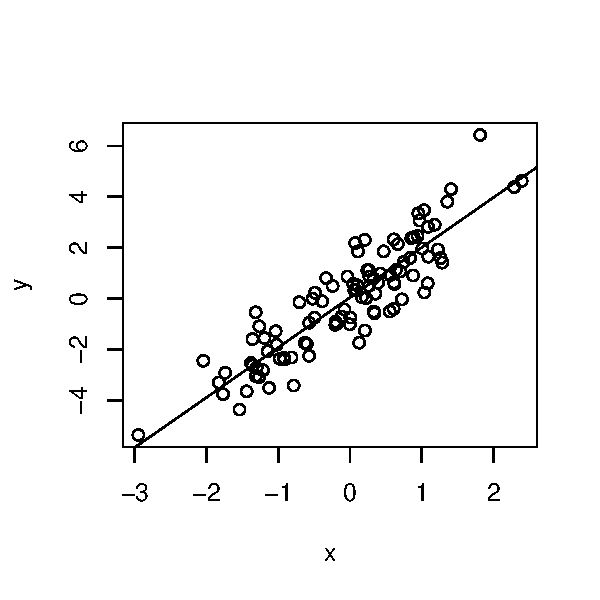
\includegraphics{manuscript_template_files/figure-latex/carDataPlot-1.pdf}
\caption{Relationship between x and y. The solid line is least-squares
linear regression.}
\end{figure}

\subsection{Citations}\label{citations}

The relationship was first described by @Halpern\_2006. However, there
are also opinions that the relationship is spurious {[}@Keil\_2012{]}.
We used R for our calculations {[}@R\_Core\_Team\_2017{]}, and we used
package \texttt{knitcitations} {[}@Boettiger\_2017{]} to make the
bibliography.

\section{Results and discussion}\label{results-and-discussion}

Lorem ipsum dolor sit amet, est ad doctus eligendi scriptorem. Mel erat
falli ut. Feugiat legendos adipisci vix at, usu at laoreet argumentum
suscipiantur. An eos adhuc aliquip scriptorem, te adhuc dolor
liberavisse sea. Ponderum vivendum te nec, id agam brute disputando mei.

Putant numquam tacimates at eum. Aliquip torquatos ex vis, mei et quando
debitis appareat, impetus accumsan corrumpit in usu. Nam mucius facilis
singulis id, duo ei autem imperdiet instructior. Cu ceteros alienum mel,
id vix putant impedit, ex idque eruditi forensibus eum. Posse dicunt id
usu. Ei iracundia constituto sed, duo ne exerci ignota, an eum unum
conceptam.

Has audire salutandi no, ut eam dicat libris dicunt. Pri hendrerit
quaerendum adversarium ea, dicat atqui munere et sea. Illum insolens eos
ne, eu enim graece rationibus mea. At postea utamur mel, eius nonumes
percipitur at vis. Numquam similique in per, te quo saepe utroque
pericula.

Ea nonumy volumus usu, no mel inermis dissentias. Dico partiendo
vituperatoribus eum et. Mea accusam convenire te, usu populo qualisque
gloriatur ut. Eu eum oratio altera option, ad mea ignota scriptorem. Ne
suas latine vix, eos oblique sanctus pertinax cu.

\section{References}\label{references}


\end{document}
